\section{KC3D: The VRML Toolbox}
As mentioned in the previous section, parametric models may be built on more
basic components which can be used in a variety of models. This section
describes these basic components and the details of their parameters. The
basic models are organized into the \verb#kc3d# module. As with many Python
modules, interactive information can be displayed about the module and
its components, for example:

\begin{verbatim}
import kc3d
help("kc3d")
help("kc3d.Polygon")
help("kc3d.Circle")
\end{verbatim}

This section aims to present the details of each component of the kc3d module
in a more intelligible fashion, but while working within the Python interpreter
the built-in information is a very helpful tool.


\subsection{kc3d.ofstream()}
This object is a simple wrapper for the C++ std::ofstream which is used as
a parameter to all routines which write data to a file. The exposed methods
are as follows:

\textbf{kc3d.ofstream.open(filename)} : opens the file with the given filename.

\textbf{kc3d.ofstream.close()} : closes the file.

\textbf{kc3d.ofstream.good()} : returns 1 if the file stream is in a good state
and 0 if there are errors.

\textbf{kc3d.ofstream.is\_open()} : returns 1 if a file is currently open.

\subsection{kc3d VRML File Operations}
There are a number of methods which can be called directly from the
kc3d module to operate on VRML files.

\textbf{kc3d.SetupVRML(filename, file)} : Open a VRML file with the given
filename and write the header information. The argument \textbf{file}
is an object of type \textbf{kc3d.ofstream()}.  Return values are
0 for success and -1 for failure.

\textbf{kc3d.SetupXForm(name, file, tabs)} : Creates the opening
text for a VRML Transform block.  The \textbf{name} is the name
of the transform, \textbf{file} is a file which was previously opened
via a call to \textbf{SetupVRML}, and \textbf{tabs} is the
formatting indentation level. Return values are 0 for success and
-1 for failure.

\textbf{kc3d.CloseXForm(file, tabs)} : Close a VRML Transform block previously
opened by a call to \textbf{SetupXForm}. Return values are 0 for
success and -1 for failure.

\textbf{kc3d.SetupShape(color, reuse, file, tabs)} : Creates the
opening text for a VRML Shape block; the text includes the 
appearance specification. The argument \textbf{color} is of
type \textbf{kc3d.VRMLMat} and it must already have loaded its
color definition from a file. If \textbf{reuse} is 1, the
Shape block will assume that the material appearance had
previously been written to the VRML file and will employ the
VRML USE directive to reuse the previous definition.
The argument \textbf{file} is an open VRML file. Return values
are 0 for success and -1 for failure.

\textbf{kc3d.CloseShape(file, tabs)} : Closes a VRML Shape block previously
opened via \textbf{SetupShape}. In a typical sequence of operations
a Shape block is opened and a geometry and coordIndex block is written
to describe a surface. Multiple Shape blocks are written to a
Transform block to describe the entire component. Return values are
0 for success and -1 for failure.

\textbf{kc3d.WriteCoord(*X, *Y, *Z, np, file, tabs)} : \textbf{*X},
\textbf{*Y}, and \textbf{*Z} are pointers to arrays containing the
coordinates of vertices and \textbf{np} is the number of vertices.
This method writes the series of coordinate points to a
coordinate block. Return values are 0 for success and -1 for failure.

\textbf{kc3d.SetupCoordIndex(file, tabs)} : Create the opening text
of a VRML coordIndex block. After opening such a block, the user
must write a list of indices defining each facet to be rendered.
Return values are 0 for success and -1 for failure.

\textbf{kc3d.CloseCoordIndex(file, tabs)} : Closes a coordIndex
block. Return values are 0 for success and -1 for failure.

\subsection{kc3d.Material() and kc3d.VRMLMat()}
The \textbf{Material} class is the representation of the VRML2.0 material
appearance as described in individual files in the project's \verb#mcad/colors#
directory. The base class is meant to hold the basic data while derived classes
implement input and output functions specific to the class of 3D models such
as VRML, Free-CAD, etc. Only the \textbf{Load} function has been exposed to
Python and it has the following form:

\textbf{Material.Load(filename)}: where the filename is the path to a
material definition file. Return values are 0 for success and -1 for failure.

The \textbf{VRMLMat} class is derived from \textbf{Material} and implements
the \textbf{Write} routine to write a VRML2.0 material appearance block to
a file:

\textbf{VRMLMat.Write(file, tabs, mainblock)}: where \textbf{file} is an open
output file of type \textbf{kc3d.ofstream()}, \textbf{tabs} is an integer
specifying the formatting indentation level, and \textbf{mainblock} is a boolean
which controls the content of the output information; if the value is 0 then
a material block appropriate for inclusion in a VRML Shape block is generated,
otherwise a material block appropriate for inclusion in the main VRML body
is generated.  Return values are 0 for success and -1 for failure.

For more information on material specifications, see the VRML2.0 specification.
The use of material specification files is encouraged to promote uniformity of
appearance between related classes of models created by different users or by
a single user at a different time. Below are the contents of a material
specification file for the appearance of the glass envelope of a DO-35 packaged
axial glass encapsulated diode:

\begin{verbatim}
# Clear glass

name: glass_clr
diffuse: 0.3 0.3 0.3
emissive: 0 0 0
specular: 0.3 0.3 0.3
ambient: 1
transparency: 0.6
shininess: 1
\end{verbatim}

\subsection{kc3d.Quat()}
The \textbf{Quat} class is the representation of a basic quaternion. It supports
multiplication and division by a scalar and addition and subtraction of quaternions
and scalars. The quaternion can be normalized by invoking the method \textbf{normalize()}
or the vector component alone can be normalized via a call to \textbf{vnormalize()}.
The individual components w, x, y, and z are publicly exposed. The cross product
and angle of two vectors can be calculated by \textbf{cross(vector\_b)} as demonstrated
in the script below. The cross product assumes a right-handed coordinate system; if
you are using a left-handed coordinate system you must multiply the pseudovector
coefficients by the appropriate unit vector coefficients.

\begin{verbatim}
import kc3d
from kc3d import *

# vector A points along the X axis
A = Quat(0, 1, 0, 0)

# vector B points along the Y axis
B = Quat(0, 0, 1, 0)

# the cross product (vector C) must point
# along the Z axis and have a rotation of pi/2
C = A.cross(B)
print C.w
print C.x
print C.y
print C.z
\end{verbatim}

\subsection{kc3d.Translation()}
The \textbf{Translation} class is the representation of data and methods to
produce a 3D geometric translation. The translation parameters can be set at any
time by invoking the methods \textbf{set(x, y, z)} or \textbf{set(q)} where \textbf{q}
is a quaternion representing the translation. A point can be
translated by invoking one of the following methods:

\textbf{translate(q)} : translate a single point represented by a quaternion

\textbf{translate(X, Y, Z)} : translate a single point

The method \textbf{isUnity()} returns 1 if the translation is an identity operation and
0 if not.

\subsection{kc3d.Rotation()}
The \textbf{Rotation} class is the representation of data and methods to produce
a 3D geometric rotation in a right-handed coordinate system. Internally the
parameters are stored as a normalized quaternion where \textbf{w} represents the
rotation in radians, and the vector component (\textbf{x}, \textbf{y}, \textbf{z})
represents the axis of rotation which passes through the coordinate origin (0, 0, 0).
The rotation parameters can be changed at any time via the methods \textbf{set(q)}
and \textbf{set(w, x, y, z)}. A point can be rotated by invoking one
of the following methods:

\textbf{rotate(q)} : rotate a single point represented by a quaternion

\textbf{rotate(X, Y, Z)} : rotate a single point

The method \textbf{isUnity()} returns 1 if the rotation is an identity operation and
0 if not.

The internal values of the rotation variable can be retrieved via \textbf{Quat get()}.

\subsection{kc3d.Scale()}
The \textbf{Scale} class is the representation of data and methods of a
a 3D geometric scaling operation.  The scale parameters can be changed at
any time via the method \textbf{set(x, y, z)}. A point can be scaled by invoking
one of the following methods:

\textbf{scale(q)} : scale a single point represented by a quaternion

\textbf{scale(X, Y, Z)} : scale a single point

The method \textbf{isUnity()} returns 1 if the scale is an identity operation and
0 if not.

\subsection{kc3d.Transform()}
The \textbf{Transform} class represents a generic 3D transformation in a right-handed
coordinate system. A transform is represented internally as a rotation, translation,
and scale operation in that order.  The parameters for all three transformation
operations can be set at any time by invoking \textbf{set(translation, rotation, scale)}.
The transformation operations can also be set individually by invoking the
following methods:

\begin{itemize}
\item \textbf{setTranslation(q)}\\
\item \textbf{setTranslation(Translation)}\\
\item \textbf{setTranslation(x, y, z)}\\
\item \textbf{setTranslation(q)}\\
\item \textbf{setRotation(q)}\\
\item \textbf{setRotation(Rotation)}\\
\item \textbf{setRotation(w, x, y, z)}\\
\item \textbf{setScale(q)}\\
\item \textbf{setScale(scalefactor)}\\
\item \textbf{setScale(Scale)}\\
\item \textbf{setScale(x, y, z)}\\
\end{itemize}

Individual points or sets of points can be transformed via the following methods:

\begin{itemize}
\item \textbf{xform(q)} transform a point\\
\item \textbf{xform(x, y, z)} transform a point\\
\item \textbf{xform(*q, np)} transform a set of \textbf{np} points\\
\item \textbf{xform(*x, *y, *z, np)} transform a set of \textbf{np} points\\
\end{itemize}

The individual geometric transforms can be retrieved via the following methods:

\begin{itemize}
\item \textbf{getTranslation(T)}\\
\item \textbf{getRotation(R)}\\
\item \textbf{getScale(S)}\\
\end{itemize}

\subsection{kc3d.Polygon()}
The \textbf{Polygon} is an abstract class implementing the methods \textbf{paint}
and \textbf{stitch} to render the faces of a convex polygon or to create facets
between the points of two polygons.

\textbf{paint(ccw, xform, color, reuse, file, tabs)} : Render the faces of a convex polygon;
ccw is a boolean which is true if vertices are to be rendered in a counterclockwise order (this
affects the side the face is visible from), xform is a transform to apply to the output vertices,
color is a VRMLMat object, and reuse is a boolean controlling the reuse of the color.
Return values are 0 for success and -1 for failure.

\textbf{stitch(ccw, polygon2, xform, color, reuse, file, tabs)} : Render facets between two
polygons. Return values are 0 for success and -1 for failure.

\textbf{extrude(cap0, cap1, outer, center, upto, xform, color, reuse, file, tabs)} : 
Render an extrusion; cap0 and cap1 determine whether each end of the extrusion is
visible, outer determines whether the outside or inside is visible, center is the
center of the polygon, upto is the vector describing the position, orientation,
and scale of the extrusion's endpoint, xform is a transform to apply to the results,
and so on. \textbf{CAVEAT: the argument \emph{outside} is not strictly the outside,
it depends on the normal of the surface relative to the transform upto.}
Return values are 0 for success and -1 for failure.

\textbf{xform(transform)} : transform the internal vertices of the polygon.

\textbf{getVertices(**x, **y, **z)} : retrieve pointers to the vertex coordinates.
The return value is an integer specifying the number of vertices; -1 may be returned
if there is a fault. [note: untested; may need reimplementation]

\textbf{isValid()} : returns 1 if the polygon contains valid vertices and 0 if not.

\textbf{clone()} : [Abstract] This method must be implemented by derived classes;
it is used to create copies of a class derived from Polygon.

\textbf{calc(x, y, xform)} : [Abstract] This method must be implemented by derived
classes. The method calculates the vertices of the polygon; x is the
maximum extent of the polygon along the X axis, y is the maximum extent
along the Y axis, and xform is a transform to be applied to the results.
For example, in the derived class Circle, x and y specify the diameter
of the ellipse along the X and Y axes.

The stitched polygons must have the same number of vertices but no other restrictions
apply.  For example, the following pyscript produces a bizarre object by stitching a
rectangle with beveled edges to an octagon inscribed within an ellipse:

\begin{verbatim}
import kc3d
from kc3d import *

rect = Rectangle()
circ = Circle()

color = VRMLMat()
color.Load("../colors/rcc_grn_g.mat")

t0 = Transform()
t1 = Transform()
t1.setTranslation(0, 0, 5)

rect.setBevel(0.5, 1)
rect.calc(8, 4, t0)

circ.setNVertices(8)
circ.calc(4, 8, t1)

out = ofstream()
SetupVRML("weird.wrl", out)
SetupXForm("WEIRD_OBJECT", out, 0)
rect.paint(False, t0, color, 0, out, 2)
rect.stitch(True, circ, t0, color, 1, out, 2)
circ.paint(True, t0, color, 1, out, 2)
CloseXForm(out, 0)
out.close()
\end{verbatim}

The following script demonstrates how the nominal outside of the
extrusion depends on the vector \emph{upto}.

\begin{verbatim}
import kc3d
from kc3d import *

rect = Rectangle()

color = VRMLMat()
color.Load("../colors/rcc_grn_g.mat")

t0 = Transform()
t1 = Transform()
t1.setTranslation(0, 0, 5)

rect.setBevel(0.5, 1)
rect.calc(8, 8, t0)
center = Quat(0, 0, 0, 0)

out = ofstream()
SetupVRML("outside_normal.wrl", out)
SetupXForm("OUTSIDE_DEMO_A", out, 0)
rect.extrude(True, True, True, center, t1, t0, color, 0, out, 2)
CloseXForm(out, 0)
out.close()

SetupVRML("outside_invert.wrl", out)
SetupXForm("OUTSIDE_DEMO_B", out, 0)
t1.setTranslation(0, 0, -5)
rect.extrude(True, True, True, center, t1, t0, color, 0, out, 2)
CloseXForm(out, 0)
out.close()
\end{verbatim}

\begin{figure}
\label{fig:k3dtools-weird}
\centering
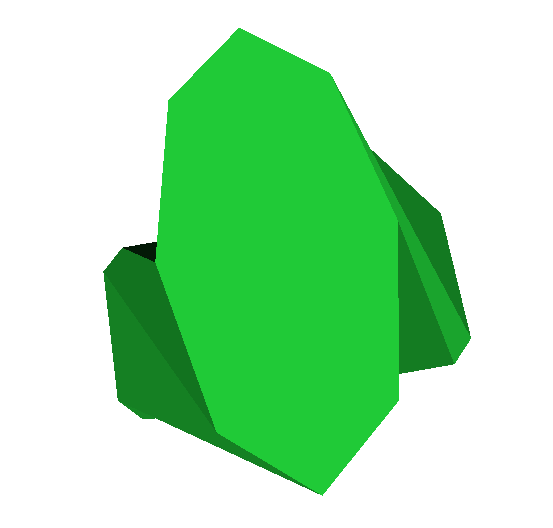
\includegraphics[width = 0.5\textwidth]{img/k3dtools-weird.png}
\caption{This is an unusual figure demonstrating the stitch operation employed on a
beveled rectangle and an octagon inscribed within an ellipse. The stitch operation
only requires that the two polygons have the same number of vertices and a polygon may
even have degenerate vertices; for example we may have an octagon which represents a point.
The vertices of a polygon object are not strictly limited to a plane but the default
paint method will only work for planar vertices.}
\end{figure}

\begin{figure}
\label{fig:k3dtools-extrude}
\centering
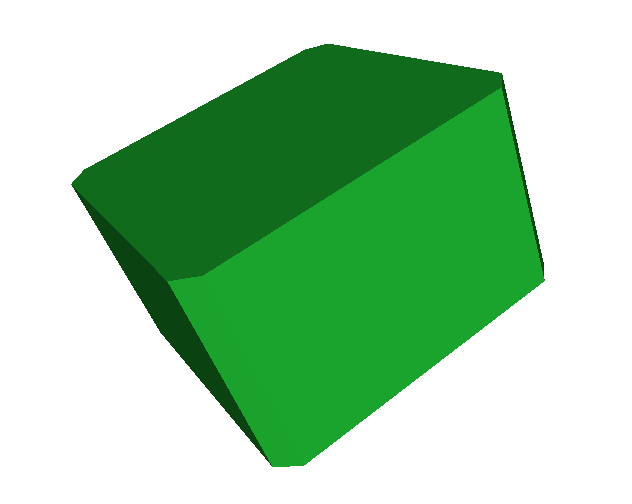
\includegraphics[width = 0.5\textwidth]{img/k3dtools-extrude.png}
\caption{A beveled polygon extruded to produce a cube.}
\end{figure}

\subsubsection{kc3d.Circle()}
\label{sec:kc3dCircle}
The \textbf{Circle} class derives from Polygon and implements a polygon of
3 to 360 vertices inscribed in an ellipse.  The more vertices, the better the approximation
to an ellipse; however, this comes at the cost of memory and file size consumed by the
model.  For an excellent representation of a circle, 48 vertices usually suffices. For
modeling small wires, 12 to 16 vertices may suffice and in some cases even 8 vertices
will produce pleasant results. The number of vertices defaults to 16 on creation
but it can be set at any time by invoking \textbf{setNVertices(n)} prior to invoking
the \textbf{calc} method to calculate the vertices.

\subsubsection{kc3d.Rectangle()}
The \textbf{Rectangle} class derives from Polygon and implements a rectangle which
may have beveled corners. The bevel can be controlled by invoking \textbf{setBevel(bevel, segments)}
before invoking the \textbf{calc} method. A bevel $\le0$ indicates the default of no bevel; segments
is a number from 1 to 360 where 1 represents a bevel and a number $>1$ represents an approximation to
a rounded corner.  The example below shows all three corner styles; it creates a green extruded
rectangle with rounded corners which has a plain black rectangular extrusion and a blue
beveled rectangular extrusion.

\begin{verbatim}
import math
import kc3d
from kc3d import *

color = VRMLMat()
color.Load("../colors/rcc_grn_g.mat")

tx = Transform()
out = ofstream()

r1 = Rectangle()
r2 = Rectangle()

r1.setBevel(1.27, 5)
r2.setBevel(1.27, 5)

r1.calc(20.32, 15, tx)

tx.setTranslation(0, 0, 1.6)
r2.calc(20.32, 15, tx)

tx.setTranslation(0,0,0)
tx.setScale(0.3937)

SetupVRML("board.wrl", out)
SetupXForm("BOARD", out, 0)

r1.paint(False, tx, color, False, out, 2)
r2.paint(True, tx, color, True, out, 2)
r1.stitch(True, r2, tx, color, True, out, 2)

r1.setBevel(0.3, 1) 
r2.setBevel(0.3, 1) 
color.Load("../colors/rcc_blu_g.mat")
tx.setScale(1)
tx.setTranslation(-5,0,1.6)
r1.calc(5, 5, tx);
tx.setTranslation(-5,0,3.6)
r2.calc(5, 5, tx);
tx.setScale(0.3937)
tx.setTranslation(0,0,0)
r2.paint(True, tx, color, False, out, 2)
r1.stitch(True, r2, tx, color, True, out, 2)

r1.setBevel(-0.3, 1) 
r2.setBevel(-0.3, 1) 
color.Load("../colors/rcc_blk_g.mat")
tx.setScale(1)
tx.setTranslation(5,0,1.6)
r1.calc(3, 3, tx);
tx.setTranslation(5,0,2.4)
r2.calc(3, 3, tx);
tx.setScale(0.3937)
tx.setTranslation(0,0,0)
r2.paint(True, tx, color, False, out, 2)
r1.stitch(True, r2, tx, color, True, out, 2)

CloseXForm(out, 0)
out.close()
\end{verbatim}

\begin{figure}
\label{fig:k3dtools-board}
\centering
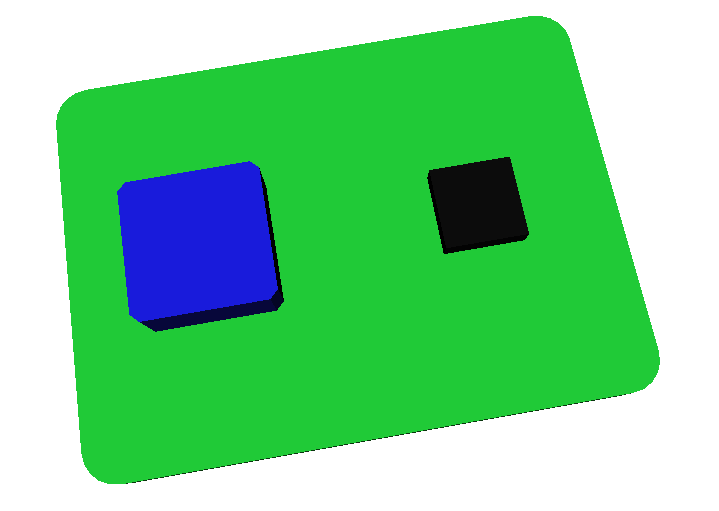
\includegraphics[width = 0.6\textwidth]{img/k3dtools-board.png}
\caption{A rectangle may be plain, as in the case of the black box, or have beveled (blue box)
or rounded corners (green board).}
\end{figure}

\subsection{kc3d.Pin()}
The \textbf{Pin} class is a representation of a vertical wire with an optional bend. The wire
may be rectangular (with or without bevels) or elliptical (see Sec.~\ref{sec:kc3dCircle} for
details about the ellipse). The starting end or both ends of the wire may be tapered, the taper
may apply to only one axis or both axes of the cross-section, and the bend may be any angle
from 0 to $\pi$ radians. 

The pin has a \textbf{calc()} method which takes a \textbf{PParams} and a Transform
argument. The members of PParams are as follows:

\begin{itemize}
\item[\textbf{w}] Pin width, X dimension\\
\item[\textbf{d}] Pin depth, Y dimension\\
\item[\textbf{h}] length of straight vertical section ($<0$ for none)\\
\item[\textbf{l}] length of straight second section ($<0$ for none)\\
\item[\textbf{bend}] bend angle, radians, $0$ to $\pi$\\
\item[\textbf{r}] bend radius, $<0$ for none\\
\item[\textbf{nb}] number of segments in a bend\\
\item[\textbf{tap}] length of tapered portion, $<0$ for none\\
\item[\textbf{dbltap}] True if both ends are to be tapered, False if only the vertical segment is tapered\\
\item[\textbf{stw}] Taper coefficient in X dimension\\
\item[\textbf{std}] Taper coefficient in Y dimension\\
\item[\textbf{bev}] bevel, applicable only to rectangular pins, $<0$ for none\\
\item[\textbf{ns}] number of vertices, applicable only to elliptical pins\\
\end{itemize}

The pin shape can be set before invoking calc via \textbf{setShape(square)} where square
is True for a rectangular pin and False for an elliptical pin; the default setting is for a
rectangular pin. The pin shape can be written to an output file via
\textbf{build(cap0, cap1, xform, color, reuse, file, tabs)} where cap0 and cap1
are booleans controlling whether or not the start and terminal ends of the pin are rendered
xform is a transformation to apply to the output data, and so on.

The example below uses two Pin objects to define the type of pin which may be found on
square pitch SMD headers:

\begin{verbatim}
import math
import kc3d
from kc3d import *

pin1 = Pin()
pin2 = Pin()

tx0 = Transform()
tx1 = Transform()
tx2 = Transform()

# set up tx0 to output to KiCAD's world scale
tx0.setScale(1.0/2.54)

# set up tx1 to lay down Pin1 and place the bottom  at Z=0
tx1.setRotation(math.pi, 1, 0, 1)
tx1.setTranslation(0, 0, 0.32)

# set up tx2 to shift the pin into position
tx2.setTranslation(4, 0, 1.32)

color = kc3d.VRMLMat()
color.Load("../colors/gold.mat")

pp0 = kc3d.PParams()
pp0.w = 0.64
pp0.d = 0.64
pp0.tap = 0.5
pp0.stw = 1
pp0.std = 0.5
pp0.dbltap = False
pp0.h = 3
pp0.r = 1
pp0.nb = 5
pp0.l = 0
pp0.bend = math.pi/2.0

pin1.calc(pp0, tx1)

pp1 = kc3d.PParams()
pp1.w = 0.64
pp1.d = 0.64
pp1.tap = -1.0
pp1.stw = 1
pp1.std = 1
pp1.dbltap = False
pp1.h = 2.44
pp1.r = 1
pp1.nb = 5
pp1.l = 5
pp1.bend = math.pi/2.0

pin2.calc(pp1, tx2)

out = kc3d.ofstream()
kc3d.SetupVRML("pindemo.wrl", out)
kc3d.SetupXForm("SMD_PIN", out, 0)
pin1.build(True, False, tx0, color, False, out, 2)
pin2.build(False, True, tx0, color, True, out, 2)
kc3d.CloseXForm(out, 0)
out.close()
\end{verbatim}

\begin{figure}
\label{fig:k3dtools-pin}
\centering
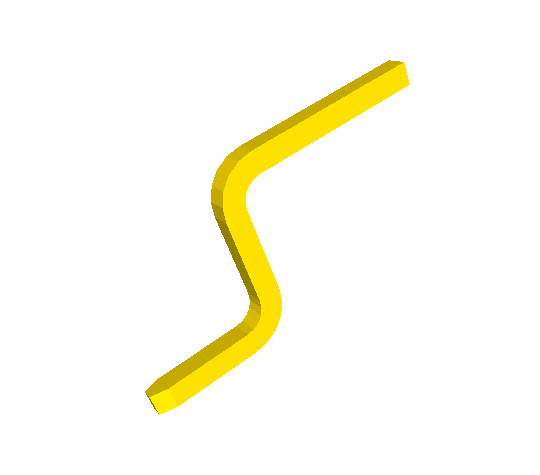
\includegraphics[width = 0.5\textwidth]{img/k3dtools-pin.png}
\caption{A pin for a typical SMD connector can be formed by superimposing
two pin objects.}
\end{figure}

\subsection{kc3d:Wire}
The class \textbf{Wire} represents a path swept with a polygon.
Vertices are added using \textbf{addPoint(q)} or \textbf{addPoint(x, y, z)}
where q is a quaternion and x, y, z represent the 3D coordinates of a point.
All points can be cleared by invoking \textbf{clear()}. The path is
rendered to a file via \textbf{build(poly, cap0, cap1, outside, tx, color, reuse, file, tabs)}
where poly is the polygon, cap0 and cap1 determine whether the ends are capped or not,
outside determines whether the wire is visible from the outside, tx is the transform
to apply to the output, color is the material appearance, reuse determines whether a
color is reused or not, file is an open output file, and tabs is the formatting
indent level.

Use wires sparingly; due to the extensive number of polygons, a wire is a costly
item. Applications of a wire include modeling an inductor and modeling the
wiring of some PCB connectors. The examples below illustrate the use of the
wire; the first example has a rectangle formed into a continuous loop with
vertices on a rectangular grid, the second shows a wire bent into an odd shape
and clearly shows how the endpoint may change orientation depending on how the
wire is bent.  The third example is a triangular helical coil; a close look at
the wire ends will reveal a change in orientation; setting the number of
vertices of the circle to 3 (triangle) rather than 8 will make the change in
orientation more obvious. Note how much memory is consumed by the coil model;
a more realistic coil model would have perhaps 24 vertices in a single twist
of the helix and would take approximately 8 times as much memory.

\begin{verbatim}
import math
import kc3d
from kc3d import *

color = VRMLMat()
color.Load("../colors/rcc_grn_g.mat")

w = Wire()
w.setParams(8,1.0)
r = Rectangle()
t0 = Transform()

r.setBevel(0.1, 1)
r.calc(1, 1, t0)

out = ofstream()
SetupVRML("wiredemo_A.wrl", out)
SetupXForm("WIRE_DEMO", out, 0)
# last leg is rendered from the wrong side
w.addPoint(0, 0, 1)
w.addPoint(0, 0, 4)
w.addPoint(4, 0, 4)
w.addPoint(4, -4, 4)
w.addPoint(0, -4, 4)
w.addPoint(0, -4, 0)
w.addPoint(4, -4, 0)
w.addPoint(4, 0, 0)
w.addPoint(1, 0, 0)
w.addPoint(0, 0, 0)
w.addPoint(0, 0, 1)
w.build(r, False, False, True, t0, color, False, out, 2)
w.clear()
CloseXForm(out, 0)
out.close()

SetupVRML("wiredemo_B.wrl", out)
SetupXForm("WIRE_DEMO", out, 0)
w.addPoint(0, 0, 0)
w.addPoint(0, 0, 4)
w.addPoint(4, 0, 4)
w.addPoint(4, -4, 4)
w.addPoint(0, -4, 4)
w.addPoint(1, -3, 0)
w.addPoint(4, -4, 0)
w.addPoint(4, -4, -3)
w.build(r, True, True, True, t0, color, False, out, 2)
w.clear()
CloseXForm(out, 0)
out.close()


# Triangular spiral
color.Load("../colors/copper.mat")
c = Circle()
c.setNVertices(8)
c.calc(1.0, 1.0, t0)
# Lead in
w.addPoint(0, 0, -5)
w.addPoint(0, 0, 0)
# Spiral
x = 1.0/3.0;
h = math.sqrt(75.0)
while x < 10:
    w.addPoint(x, 5, 0)
    x += 1.0/3.0
    w.addPoint(x, 0, h)
    x += 1.0/3.0
    w.addPoint(x, -5, 0)
    x += 1.0/3.0

# Lead out
w.addPoint(x, 0, 0)
w.addPoint(x, 0, -5)
SetupVRML("wiredemo_C.wrl", out)
SetupXForm("WIRE_DEMO", out, 0)
w.build(c, True, True, True, t0, color, False, out, 2)
w.clear()
CloseXForm(out, 0)
out.close()
\end{verbatim}

\begin{figure}
\label{fig:k3dtools-coil}
\centering
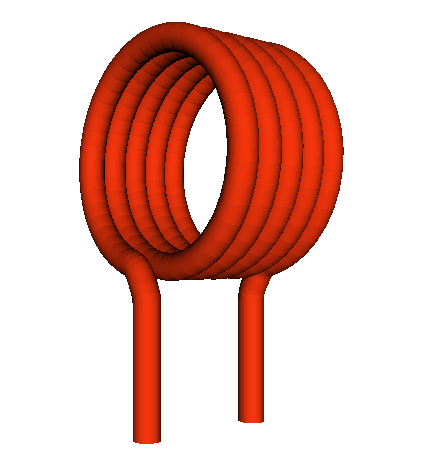
\includegraphics[width = 0.5\textwidth]{img/k3dtools-coil.png}
\caption{The wire model can be used to create objects such as an inductor. Care must be taken
when using the wire model because the resulting file may be very large; the model shown
has a file size of almost 2MB.}
\end{figure}

\subsection{kc3d.Funnel()}
The \textbf{Funnel} class is a representation of a rectangular or elliptical funnel typical
of the pin recesses in a connector. The default shape of the funnel is rectangular but the
shape can be set by invoking \textbf{setShape(square, bevel)} where \textbf{square} is True for
a rectangular funnel and \textbf{bevel} is the bevel to use on the rectangular section; use
a bevel value $<0$ for a plain rectangle.

The vertices are calculated by invoking \textbf{calc(w1, d1, w2, d2, h1, h2, h3, xform, ns)}
where w1 and d1 are the X and Y dimensions of the top of the flute, w2 and d2 and the
dimensions of the stem, h1 is the height of the flute, h2 is the height of the segment of
the stem which is the same color as the flute (this may be set to 0), and h3 is the
height of the stem segment which will be colored with stemcolor.

The shape is written to an output file by invoking \textbf{build(cap, xform, flutecolor,
reuse\_flute, stemcolor, reuse\_stem, file, tabs)} where cap is a boolean controlling
whether or not the bottom end of the stem is rendered, flutecolor is a VRMLMat object
specifying the color of the flute and the stem segment h2, reuse\_flute is a boolean
controlling the reuse of flutecolor, stemcolor is a VRMLMat object specifying the color
of the h3 section of the stem, and reuse\_stem controls the reuse of the stem color.

The example below creates a funnel with a blue beveled flute and golden stem:

\begin{verbatim}
import kc3d
from kc3d import *

tx = Transform()

fun = Funnel()
fun.setShape(True, 0.2)
fun.calc(1.6, 1.6, 0.96, 0.96, 0.5, 0.2, 3, tx, 24)

fcolor = kc3d.VRMLMat()
fcolor.Load("../colors/rcc_blu_g.mat")

scolor = kc3d.VRMLMat()
scolor.Load("../colors/gold.mat")

out = kc3d.ofstream()
kc3d.SetupVRML("funneldemo.wrl", out)
kc3d.SetupXForm("FUNNEL_DEMO", out, 0)
fun.build(True, tx, fcolor, False, scolor, False, out, 2)
kc3d.CloseXForm(out, 0)
out.close()
\end{verbatim}

\begin{figure}
\label{fig:k3dtools-funnel}
\centering
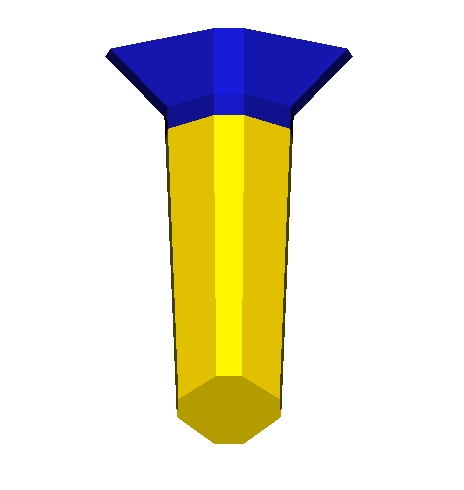
\includegraphics[width = 0.5\textwidth]{img/k3dtools-funnel.png}
\caption{A square funnel typical of female header connectors. The funnel model
can also produce circular funnels and more esoteric shapes such as rectangular
and elliptical funnels.}
\end{figure}

\subsection{kc3d.Hole()}
The \textbf{Hole} class represents a plain rectangular panel with a rectangular or elliptical
hole in it; a rectangular hole may be beveled. A hole may be used to surround the flute of a
funnel or to provide thru-holes for pins.

The vertices are calculated by invoking \textbf{calc(w1, d1, w2, d2, tx, square, off\_x, off\_y, np, bev)}
where w1 and d2 are the X and Y dimensions of the frame, w2 and d2 are the dimensions of the
hole, square specifies a rectangular hole when set to True, off\_x and off\_y are offsets of
the hole, np is the number of vertices in a circular hole and bev is the optional bevel of
a rectangular hole (set bev to -1 if you do not want a bevel).

The shape information is written to a file by invoking \textbf{build(xform, color, reuse, file, tabs)}.

\subsection{kc3d.Shoulder()}
The \textbf{Shoulder} class represents a rectangular extrusion which may have one rounded edge
and which may have ends which taper. A shoulder may be found, for example, as a spacer on the
bottom of header cases.

Vertices are calculated by invoking \textbf{calc(l, h, w, t, r, xform)} where l and h are the length
and height of the shoulder, w is the depth, and r is the radius of the lower inner edge ($<0$ for no radius).

The shape information may be written by invoking \textbf{build(xform, color, reuse, file, tabs)}.

\subsection{kc3d.Hdrbase()}
The \textbf{Hdrbase} class is a generic case for a square-pitch header. The case is rectangular but
may be beveled between each column of pins, the holes for the pins may be square or circular, the
holes may be a different size on the top and bottom, and the part may have a rectangular shoulder.

Case parameters are specified by invoking \textbf{setParams(xpitch, ypitch, bevel, height, sh, hassh, hd0,
hdy, hd1, squarebot, squaretop, male, pbev, fbev, columns, rows, ns)}:

\begin{itemize}
\item \textbf{xpitch}: pin pitch along the X axis (columns)
\item \textbf{ypitch}: pin pitch along the Y axis (rows)
\item \textbf{bevel}: bevel between columns ($<0$ for none)
\item \textbf{height}: overall height of the case (measured from the top of the PCB)
\item \textbf{sh}: shoulder height ($<0$ for none); this is the gap between the top of the PCB and the bottom of the header
\item \textbf{hassh}: set True if a shoulder is to be rendered; otherwise the sh parameter simply produces a gap
\item \textbf{hd0}: X dimension of the bottom hole (if the hole is circular, the Y dimension will be set equal to hd0)
\item \textbf{hdy}: Y dimension of the bottom hole; applicable only if the hole is rectangular
\item \textbf{hd1}: dimension of the top hole; the top hole is constrained to a square or circle if the case type is
    for a female header and if the case is for a male header the top hole dimensions are the same as the bottom
    hole dimensions
\item \textbf{squarebot}: set True if the bottom pins are square or rectangular
\item \textbf{squaretop}: set True if the top holes are square (applicable only for female headers)
\item \textbf{male}: set True if the case is for a male header
\item \textbf{pbev}: bevel of the bottom hole; applicable only if squarebot is True
\item \textbf{fbev}: bevel of the top hole; applicable only if male is False and squaretop is True
\item \textbf{columns}: number of columns; valid range is $\ge1$
\item \textbf{rows}: number of rows; valid range is $\ge1$
\item \textbf{ns}: number of vertices to use for circular pins
\end{itemize}

The shape information is written to a file by invoking \textbf{build(xform, color, reuse, file, tabs)}.
The example below creates a beveled 6x2 header case suitable for a vertical female header with square pins.
Notice that the case does not include any features such as a funnel on the top holes since such features
are specific to individual header models; for example the Genhdr model may place one of at least three
different features into the top holes.

\begin{verbatim}
import kc3d
from kc3d import *

hdr = Hdrbase()
tx0 = Transform()

# set up tx0 to output to KiCAD's world scale
tx0.setScale(1.0/2.54)

color = kc3d.VRMLMat()
color.Load("../colors/rcc_blu_g.mat")

hdr.setParams(2.54, 2.54, 0.3, 8, 0.72, True, 0.64, 0.64, 1.6, True, True, False, -1, -1, 6, 2, 24)

out = kc3d.ofstream()
kc3d.SetupVRML("hdrcasedemo.wrl", out)
kc3d.SetupXForm("HEADER_CASE_DEMO", out, 0)
hdr.build(tx0, color, False, out, 2)
kc3d.CloseXForm(out, 0)
out.close()
\end{verbatim}

\begin{figure}
\label{fig:k3dtools-hdrcase}
\centering
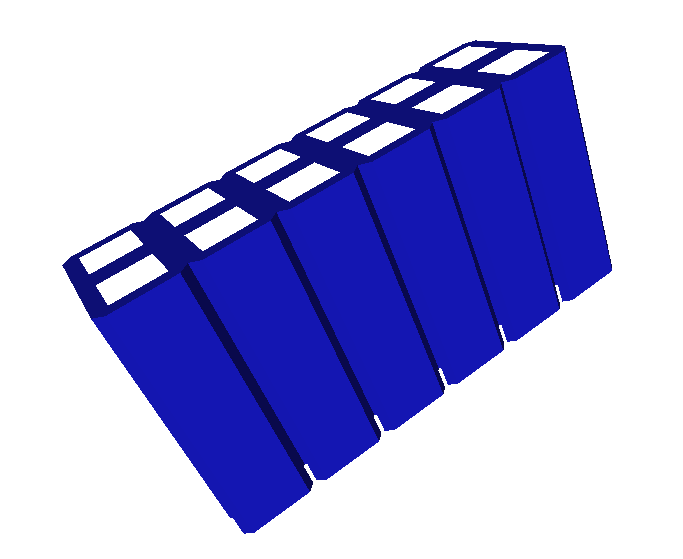
\includegraphics[width = 0.6\textwidth]{img/k3dtools-hdrcase.png}
\caption{A sample of a header casing suitable for a female header connector.
The multiple holes on the top are rendered by the Hole object.}
\end{figure}
